\documentclass{beamer}
\usepackage[latin1]{inputenc}
\usepackage{amsfonts}
\usepackage{array}
%\usepackage{verbatim}
%\usetheme{Luebeck}
\usetheme{Warsaw}
\title[Kinect Controlled Robotic Arm]{Kinect Controlled Robotic Arm}
%\subtitle{CS308 Project Presentation I}

\author {CS308 Project - 2012}
\date{Group 10}
\begin{document}
\begin{frame}
\titlepage


\begin{tabular}{lllll}
Aakash Rao N S & (09005069) & & Aayush Singhal &  (09005041) \\
Sivakanth Gopi  &  (09005043) & & Sriram Bhragav K &  (09005067)\\\
\end{tabular}\\

\begin{center}
under the guidance of\\
Prof. Kavi Arya
\end{center}
\end{frame}

\section{Problem Statement and Description}
\subsection{Motivation}
\begin{frame}{Motivation}
\begin{itemize}
\item[-] Controlling a robotic arm with a traditional controller can be very difficult
\item[-] Non-intuitive and increases the complexity of operation
\end{itemize}
What we need is a Natural User Interface (NUI)
\begin{itemize}
\item[-] With NUI the human arm can directly control the robotic arm which tries to imitate its movements
\item[-] Thus controlling the arm becomes very intuitive 
\item[-] Opens a plethora of applications
\end{itemize}
\end{frame}


\subsection{Problem Statement}
\begin{frame}{Problem Statement}
Provide a NUI for remotely controlling  a robotic arm
\begin{itemize}
\item[-] robotic arm should imitate the movements of the user arm
\item[-] use kinect to capture human arm movements
\item[-] develop an algorithm to convert human arm movements into robotic arm movements in a way that makes the control intuitive
\end{itemize}
\end{frame}

\subsection{Description}
\begin{frame}{Description}
\begin{itemize}
\item[-]user moves his arms to control the arm
\item[-]movements and gestures of human arm are captured using kinect which are sent to the controller (computer)
\item[-]the controller uses an algorithm to convert this movements into movements of robotic arm
\item[-]robotic arm imitates the the movements of the human arm
\item[-]user can monitor his movements in a GUI
\end{itemize}
\end{frame}

\section{Functional Requirements and Execution}
\subsection{Functional Requirements}
\begin{frame}{Functional Requirements}
\begin{enumerate}
\item Robotic Arm
\begin{itemize}
\item The robotic arm should have sufficient degrees of freedom to accurately  imitate the human arm
\item The response time of the robotic arm should be less to provide fast real time movement
\end{itemize}
\item 3D capturing device
\begin{itemize}
\item The device should capture the 3D positions of the joints of the human arm in real time
\item It should have a decent of frame rate of atleast 15 fps
\end{itemize}
\end{enumerate}
\end{frame}   

\subsection{Work Execution}
\begin{frame}{Work Execution (1/2)}
\begin{itemize}
\item Develop an API for controlling the robotic arm (2 days)
\item Develop Kinect interface and some related classes for getting positions of human arm joints and required angles(1 day)
\item Mapping each axes of the robotic arm to those of human arms, testing and fine tuning(1 day)
\item Developing and implementing an improved algorithm for providing an much more intuitive user control (3 days)
\end{itemize}
\end{frame}

\begin{frame}{Work Execution (2/2)}
\begin{itemize}
\item Testing the new algorithm and fine tuning of various parameters (1 day)
\item Documenting and cleaning code, making final presentation and video script (2 days)
\end{itemize}
\end{frame}

\subsection{Work Division}
\begin{frame}{Work Division}
\begin{table}[h]
\setlength{\tabcolsep}{10pt}
%\centering
\noindent\makebox[\textwidth]{
\begin{tabular}{|m{0.4\textwidth}|m{0.4\textwidth}|}
\hline
\textbf{Work/Critical Tasks}& \textbf{People Responsible} \\
\hline
Module for Real Time Serial Port Communication with the arm& Aakash, Gopi, Bhargav\\
\hline
Module for Handling Sekletal Data and Performing Calculations & Aayush, Gopi, Bhargav\\
\hline
Design and Coding of the Two-Circle Algorithm & Gopi, Aayush, Aakash\\
\hline
Graphical User Interface (GUI) for the Application & Bhargav, Aayush, Gopi\\
\hline
Documentation & All\\
\hline
\end{tabular}}
\end{table}
Project Completion Date : 19th April 2012
\end{frame}


\subsection{Finite State Machine}
\begin{frame}{GUI FSM}
\begin{figure}
\centerline{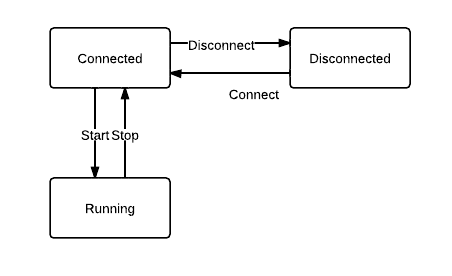
\includegraphics[scale=0.7]{images/guifsm.png}}
\caption{Service Bot FSM}\label{fig:exp}
\end{figure}
\end{frame}

\section{Innovations, Challenges and Solutions}
\subsection{Innovations and Challenges}
\begin{frame}{Innovation and Challenges}
\begin{itemize}
\item Developing an API for robotic arm control 
\item Designing an intuitive control mechanism for the user
\item Developing an efficient algorithm for finding the angles of the robotic arm
\item Implementing some averaging features to remove deviations in the kinect data
\end{itemize}
\end{frame}


\subsection{Problems and Solutions}
\begin{frame}{Problems and Solutions(1/3)}
\begin{itemize}
\item API/Hardware manual for robotic arm not available
\begin{itemize}
\item[-] decompiled the robotic arm control GUI, read and understood the code and developed an API/library which future projects can use
\end{itemize}
\item Kinect cannot capture finger and wrist movements
\begin{itemize}
\item[-] use the left arm to intuitively control the wrist and pinch motors
\end{itemize}
\end{itemize}
\end{frame}   

\begin{frame}{Problems and Solutions(2/3)}
\begin{itemize}
\item Kinect data contains many disturbances and leads to the arm deviating unnecessarily
\begin{itemize}
\item[-] used the median of the last few values to remove extremes. Number of samples used shouldn't be too less or too high, 10 seemed a good value after testing
\end{itemize}
\end{itemize}
\end{frame}   

\begin{frame}{Problems and Solutions(3/3)}
\begin{itemize}
\item Human arm and the robotic arm are structurally very different
\begin{itemize}
\item[-] initially performed a direct angle-to-angle mapping from the human arm to the robotic arm, but it was not very intuitive
\begin{figure}
\centerline{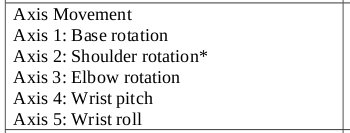
\includegraphics[scale=0.4]{images/arm-axes-table.jpg}}
\caption{Direct Mapping of Angles}
\end{figure}
\item[-] developed an algorithm for mapping human arm positions to the positions of the robotic arm (most difficult part)
\end{itemize}
\end{itemize}

\end{frame}


\begin{frame}{Algorithm - Problem}
  We will basically aim to keep the hand of the robotic arm in the same 3D position as the human hand relative to the body. The angles at each axis of the robotic arm are automatically generated by the algorithm
  \begin{itemize}
  \item[-] the angles found by the algorithm should continuously vary with the position of the human hand, to ensure that the movement of the robotic arm  is smooth
  \item[-] the algorithm should find a solution whenever it exists
  \end{itemize}
\end{frame}

\begin{frame}{Algorithm - Solution}
  \begin{itemize}
  \item Rotate the base angle so that the robotic arm lies in the same vertical plane as the point we intend to reach
  \item In this plane the arm looks as shown in the figure:
  \end{itemize}
  \begin{figure}
\centerline{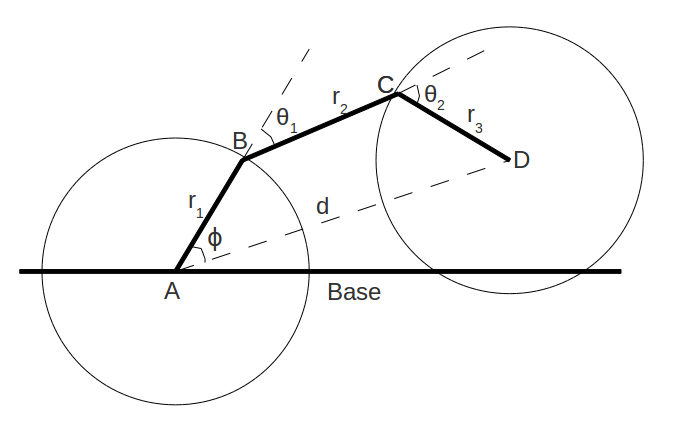
\includegraphics[scale=0.2]{images/twocircles.png}}
\caption{Two Circle Algorithm}
\end{figure}
\end{frame}

\begin{frame}{Algorithm - Solution}
  \begin{itemize}
  \item We should find $\phi,\theta_1,\theta_2$ under the constraints: $Ad=d,AB=r_1,BC=r_2,CD=r_3,-\frac{\pi}{2}\le\phi,\theta_1,\theta_2\le\frac{\pi}{2}$
  \item Observe that minimum value of $BC$ occurs when $\theta_1=\theta_2=0$ and maximum value of BC occurs when $\theta_1=\theta_2=\frac{\pi}{2}$(when BC is the direct common tangent for the two circles)
  \item So there will always exist a solution where $\theta_1=\theta_2=\theta$ and $0\le\theta\le\frac{\pi}{2}$
  \item Moreover $BC$ will be a monotonic and continuous function of $\theta$, so we can do a binary search for the solution where $BC=r_2$
  \item If $r_2>max\ BC$ then $\theta=\frac{\pi}{2}$ and if $r_2<min\ BC$ then $\theta=0$
  \end{itemize}
\end{frame}

\section{Testing Strategy}

\subsection{Modular Testing}
\begin{frame}{Modular Testing}
\begin{itemize}
\item Testing the API/library for real time serial port communication with the arm.\item Microsoft Visual Studio Professional 2010
\item Kinect for Windows SDK v1
\item .NET Framework 4.0 or higher
\item FT232 USB to Serial Converter (provided with the source)

\item Testing the skeletal data obtained using Kinect.
\item Testing the calculated angles and lengths required for the Two Circle Algorithm.
\item Testing the output of the Two Circle Algorithm.
\end{itemize}
\end{frame}

\subsection{Combined Testing}
\begin{frame}{Combined Testing}
\begin{itemize} 
\item Testing the intuitiveness of the control by asking subjects to try to pick and place objects using the arm.
\item Testing the GUI for application, which is controls and connection various parameters.
\item Testing the effect of modifying various parameters of the algorithm and selecting the ones that give the best results.
\end{itemize}
\end{frame}

\subsection{Performance Metrics}
\begin{frame}{Performance Metrics}
\begin{itemize}
\item The servo motors have response time of somewhere between 0.5 - 1.0 s. This is leads to a delay in the response produced and takes some time to get used to.
\item We asked 10 random subjects to try to pick and place a block. The average time taken by them to complete the task was recorder. This is a measure of the intuitiveness of the algorithm. It was found to be around 40 - 60 seconds.  
\end{itemize}
\end{frame}

\section{Code Reusability}
\begin{frame}{Code Reusability}
Modular Design:
\begin{itemize}
\item[-] modules independent of each other, hence can be changed without changing others
\item[-] developed an API/library for robotic arm control which future projects can use
\item[-] the algorithm for finding the arm angles also has wrappers which can  be reused
\end{itemize}
\end{frame}

\section{Future Directions}
\begin{frame}{Future Directions}
\begin{itemize}
\item A more sophisticated algorithm using quaternions and some mechanism for stabilising against disturbances could be the next direction of the project
\item The arm can be remotely deployed by communicating through ZigBee and mounting a camera near the arm
\item An arm with a faster response time can be reduced to make the control much more intuitive
\end{itemize}
\end{frame}

\end{document}
